\section{Testing of the Project}

\subsection{Functional Testing}
{\color{red}
	\begin{itemize}
		\item In this section, each of the functional requirements laid out in section \ref{sec:funcs} have been evaluated in turn, to ensure the system meets them. Knowledge of the inner workings of the system is not actually necessary to understand these tests, as they simply check whether functionality is present, and are not concerned as to how the system actually implements it (this is known as black box testing \cite{beizer1995black}). A complete listing of all the tests conducted, and their results, can be found in appendix \ref{app-ctl}.\ \\
		\ \\
		some interesting thing to point out... ?
	\end{itemize}
}

\subsection{Non-Functional Testing}
{\color{red}
	\begin{itemize}
		\item Look at non-functional requirements and talk about if they were met
		\item Just like last year's diss
	\end{itemize}
}
\paragraph{Accessibility}\ \\
{\color{red} What this met? If so, \textbf{how}?}

\paragraph{Usability and Operability}\ \\
{\color{red} What this met? If so, \textbf{how}?}

\paragraph{Maintainability \& Documentation}\ \\
{\color{red} What this met? If so, \textbf{how}?}

\paragraph{Quality}\ \\
{\color{red} What this met? If so, \textbf{how}?}

\paragraph{Resource Requirements and Constraints}\ \\
{\color{red} What this met? If so, \textbf{how}?}

\paragraph{Cross Platform Compatibility}\ \\
{\color{red} What this met? If so, \textbf{how}?}

\paragraph{Security}\ \\
{\color{red} What this met? If so, \textbf{how}?}

\paragraph{Disaster Recovery}\ \\
{\color{red} What this met? If so, \textbf{how}?}


\newpage 
\subsection{User Feedback Testing}
Usability testing is the process of getting actual users to use the system, with these users performing a set of tasks whilst being observed. The time taken to complete the various tasks, and any comments or criticisms the user had were recorded, as well as any bugs the user encountered. The purpose of these tests was to discover usability problems in the interface, and what could be made simpler.\ \\
\ \\
For the tests a sample of 15 users were selected, with a skill level ranging from low, to very high, with ages ranging from 21 to 46. The reason for this broad range was that users of different skill levels, and different ages, use and understand computers differently, and therefore what is considered intuitive for one user is not necessarily considered the same by others. This meant that the number of usability issues and simplifications that could be identified was greatly increased. The five tasks that the users were expected to complete are given below, and a full list of instruction can be found in appendix \ref{sec:utis}.

\begin{enumerate}
	\item Search for a route, and view it's details
	\item Create an account for the system
	\item Comment, rate and download a route 
	\item Create a route
	\item Navigate back to their route, and make edits
\end{enumerate}
\noindent 
These five tasks represented the five core tasks that users of Niceway.to would be expected to engage in on a regular basis (except signing up, which would only occur once, but was a barrier for entry so it was important it was short and simple). This meant it was vital that they were easy to understand, and easy to complete by users of all skills levels. It was for this reason that the instructions for the tests were as vague as possible, as not to lead the users to the correct answers. Some of these tasks were purposefully extremely simple and short, so that users could really focus on the specific areas of the system, and therefore identify more issues.\ \\
\ \\
The RITE method (Rapid Iterative Testing and Evaluation) was employed during the usability tests to quickly iterate on user feedback to fix issues with the system. This meant that, after each user completed the set of tasks, their feedback would be implemented, and any bugs they discovered would be fixed before the start of the next test. This meant that each participant would be looking at a slightly different product, and they would all be able to identify unique issues instead of being focused on the same issue.

\begin{figure}[!ht]
	\begin{center}
%		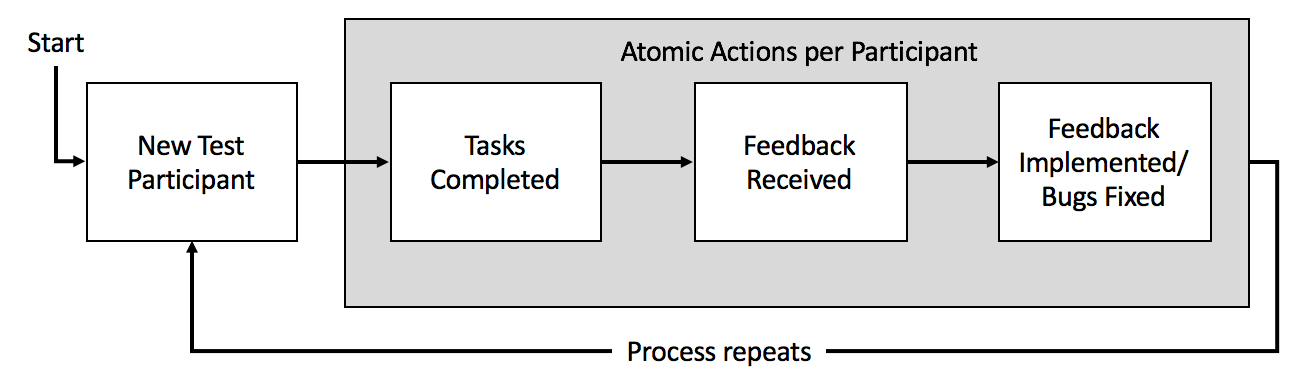
\includegraphics[width=0.9125\textwidth]{images/testing/rite.png}
	\end{center}
		{\color{red}
			diagram showing user being tested $->$ feedback $->$ iterate / change product $->$ repeat
		}
	\vspace{-3mm}
	\caption{The employed RITE method life cycle}	
\end{figure}

\newpage
\noindent
The times taken for all participants to complete each the tasks can be found in appendix \ref{sec:trfut}, with a summary presented below, and an discussion of these results forthwith.

\begin{figure}[!ht]
	\begin{center}
		%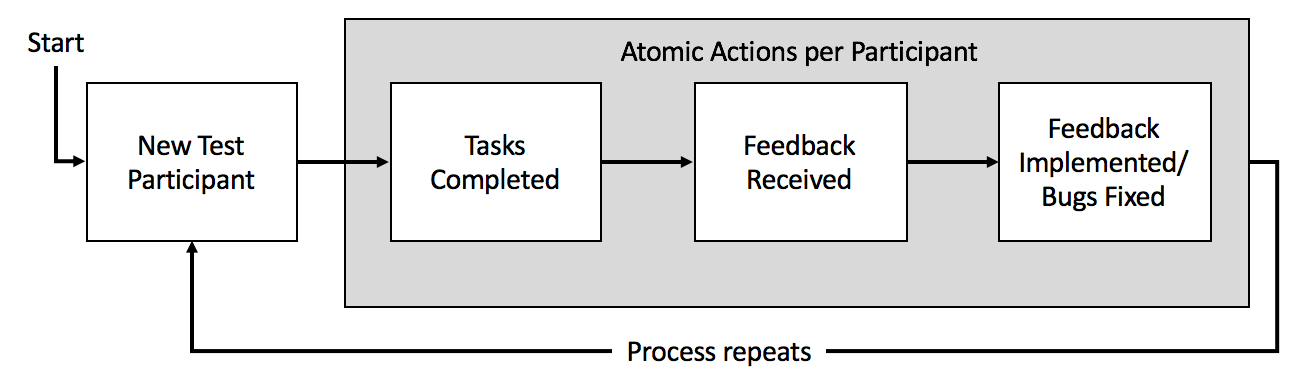
\includegraphics[width=0.9125\textwidth]{images/testing/rite.png}
	\end{center}
	{\color{red}
		
		Bar chart of min/max/average time taken to complete each task against one another. (on seperate plots) 
	}
	\vspace{-6mm}
	\caption{Summarised results from user testing}	
\end{figure}

{\color{red}
\noindent
While the numbers themselves are not necessarily important, the range of these values is. This is the different between the fastest user, and the slowest user. This range shows how difficult or simple the task is. If a task has a large range, it means the skill gap is a major factor in how to use the feature. This means that either the task is difficult, or there are shortcuts that advanced users utilised to complete the task quicker. {\color{blue}What did I do as a result of this?}. Specifically talk about each of the tasks and why the results were as they were.
}
\ \\
\ \\
{\color{red}
\noindent
The issues that were identified during the usability tests, and were then resolved in between testing stages, have been listed below. The advantage of resolving these issues in between tests is that subsequent participants will be able to detect unique and novel issues, rather than each user identifying the same set of issues.
\ \\
\ \\
\begin{tabular}{l}
	Issue Identified \\
	\hline 
	Could not press 'Return' to search on the search page\\
	Couldn't click on title on search results page\\
\end{tabular}
}
\ \\
\ \\
{\color{red} ask max ethics for this type of testing}\ \\



	